
\documentclass[11pt]{article}
\usepackage{amsmath}
\usepackage{graphicx}

\newcommand{\bv}[1][]{e_{#1}}
\newcommand{\bp}[2]{(#1,#2)}

\newtheorem{theorem}{Theorem}[section]

\graphicspath{{BasisCrossProductIllustrations/}}

\begin{document}

\title{Bivector Bases and Cross Products}
\author{Ross L. Hatton}
\date{\today}
\maketitle

A bivector basis is an ordered pairing of pairs of basis vectors. Each pair of vector basis elements forms an oriented area basis element. These basis elements are used in applications such as fluid dynamics, where they provide the signs of flux passing through test surfaces, and for defining rotations in higher dimensions (also finite element solvers)

Closely related to the question of constructing cyclic bivector bases on a space is the question of constructing a vector cross product on a space. 

\section{Cyclic Bivector Bases}


A cyclically oriented bivector basis is one in which the area basis elements are symmetric with respect to cyclic permutation of the basis elements. For example, consider a vector basis $\bv[a]$, $\bv[b]$, $\bv[c]$, which we will initially label as $\bv[1]$, $\bv[2]$, $\bv[3]$. 


The right-hand rule for three-dimensional spaces defines positive pairings to be $\bp{\bv[1]}{\bv[2]}$, $\bp{\bv[2]}{\bv[3]}$, and $\bp{\bv[3]}{\bv[1]}$, such that for our initial basis numbering the absolute pairs $\bp{\bv[a]}{\bv[b]}$, $\bp{\bv[b]}{\bv[c]}$, and $\bp{\bv[c]}{\bv[a]}$ are all positive. If we relabel each vector basis from $\bv[i]$ to $\bv[i+1]$ (so that $\bv[a]$ becomes $\bv[2]$, etc.,), the vector pairings $\bp{\bv[1]}{\bv[2]}$, $\bp{\bv[2]}{\bv[3]}$, and $\bp{\bv[3]}{\bv[1]}$ again make $\bp{\bv[a]}{\bv[b]}$, $\bp{\bv[b]}{\bv[c]}$, and $\bp{\bv[c]}{\bv[a]}$ all positive.



In contrast, the lexigraphical construction for a bivector basis from an ordered vector basis defines a bivector as positive if the first vector has a lower index number than the second basis vector, such that $\bp{\bv[1]}{\bv[2]}$, $\bp{\bv[1]}{\bv[3]}$, and $\bp{\bv[2]}{\bv[3]}$ are defined as positive, which makes $\bp{\bv[c]}{\bv[a]}$ negative. This basis is not cyclical: if we relabel $\bv[i]$ to $\bv[i+1]$, $\bp{\bv[c]}{\bv[a]}$ becomes the positive $\bp{\bv[1]}{\bv[2]}$, and $\bp{\bv[b]}{\bv[c]}$ becomes the negative $\bp{\bv[3]}{\bv[1]}$.




In the development of numerical computational tools, it is common to progress from two-dimensional to three-dimensional and then n-dimensional implementations. In moving from two dimensions to three dimensions, especially in physically-motivated problems, it is common to extend the single-element bivector basis (e1, e2) to three dimension using the right hand rule described above. The next step, moving to general n-dimensional formulations then poses a problem: How to extend the right-hand-rule basis to four or more dimensions. After some trial and error, it becomes clear to the student that there is no satisfactory way to make this extension, and they convert to a lexigraphic ordering (which requires careful examination of the project to ensure that all assumptions of a right-hand rule are replaced with the lexigraphic rule).

It is not immediately apparent, however, \emph{why} we cannot extend the right hand rule to four dimensional spaces. Our first theorem in the paper addresses this point:



\begin{theorem}{Cyclically oriented bases can only be constructed on odd-dimensional spaces.}

Proof: An oriented basis on $n$-dimensional space corresponds to a directed complete graph with $n$ nodes. Cyclic orientation with respect to an ordering of the nodes additionally requires that this graph be rotationally symmetric. A necessary condition for rotational symmetry is that there are no sources or sinks in the graph, i.e., that the graph contains (equivalently, that its edges can be induced by) an Eulerian circuit through the $n$ nodes. As per Euler’s theorem, this condition is only possible in a graph with an even number of edges on each node; for a complete graph, this means that there must be an odd number of nodes, and thus that it must correspond to an odd-dimensional space.

\end{theorem}


Some geometric intuition in support of the above proof: The complete graph on an ordered $n$-node space consists of the polygon defined by the nodes and all of its inscribed stars, as illustrated in Fig.~\ref{fig:polygonandstars}. On odd-dimensional spaces, this graph can be made into a rotationally-symmetric directed graph by assigning a traversal direction to the polygon and each of the stars. On even-numbered spaces, one of the stars is degenerate (cross-shaped) and cannot be followed without retracing another segment, so no symmetric graph can be constructed.

\begin{figure}[tbp]
\begin{center}
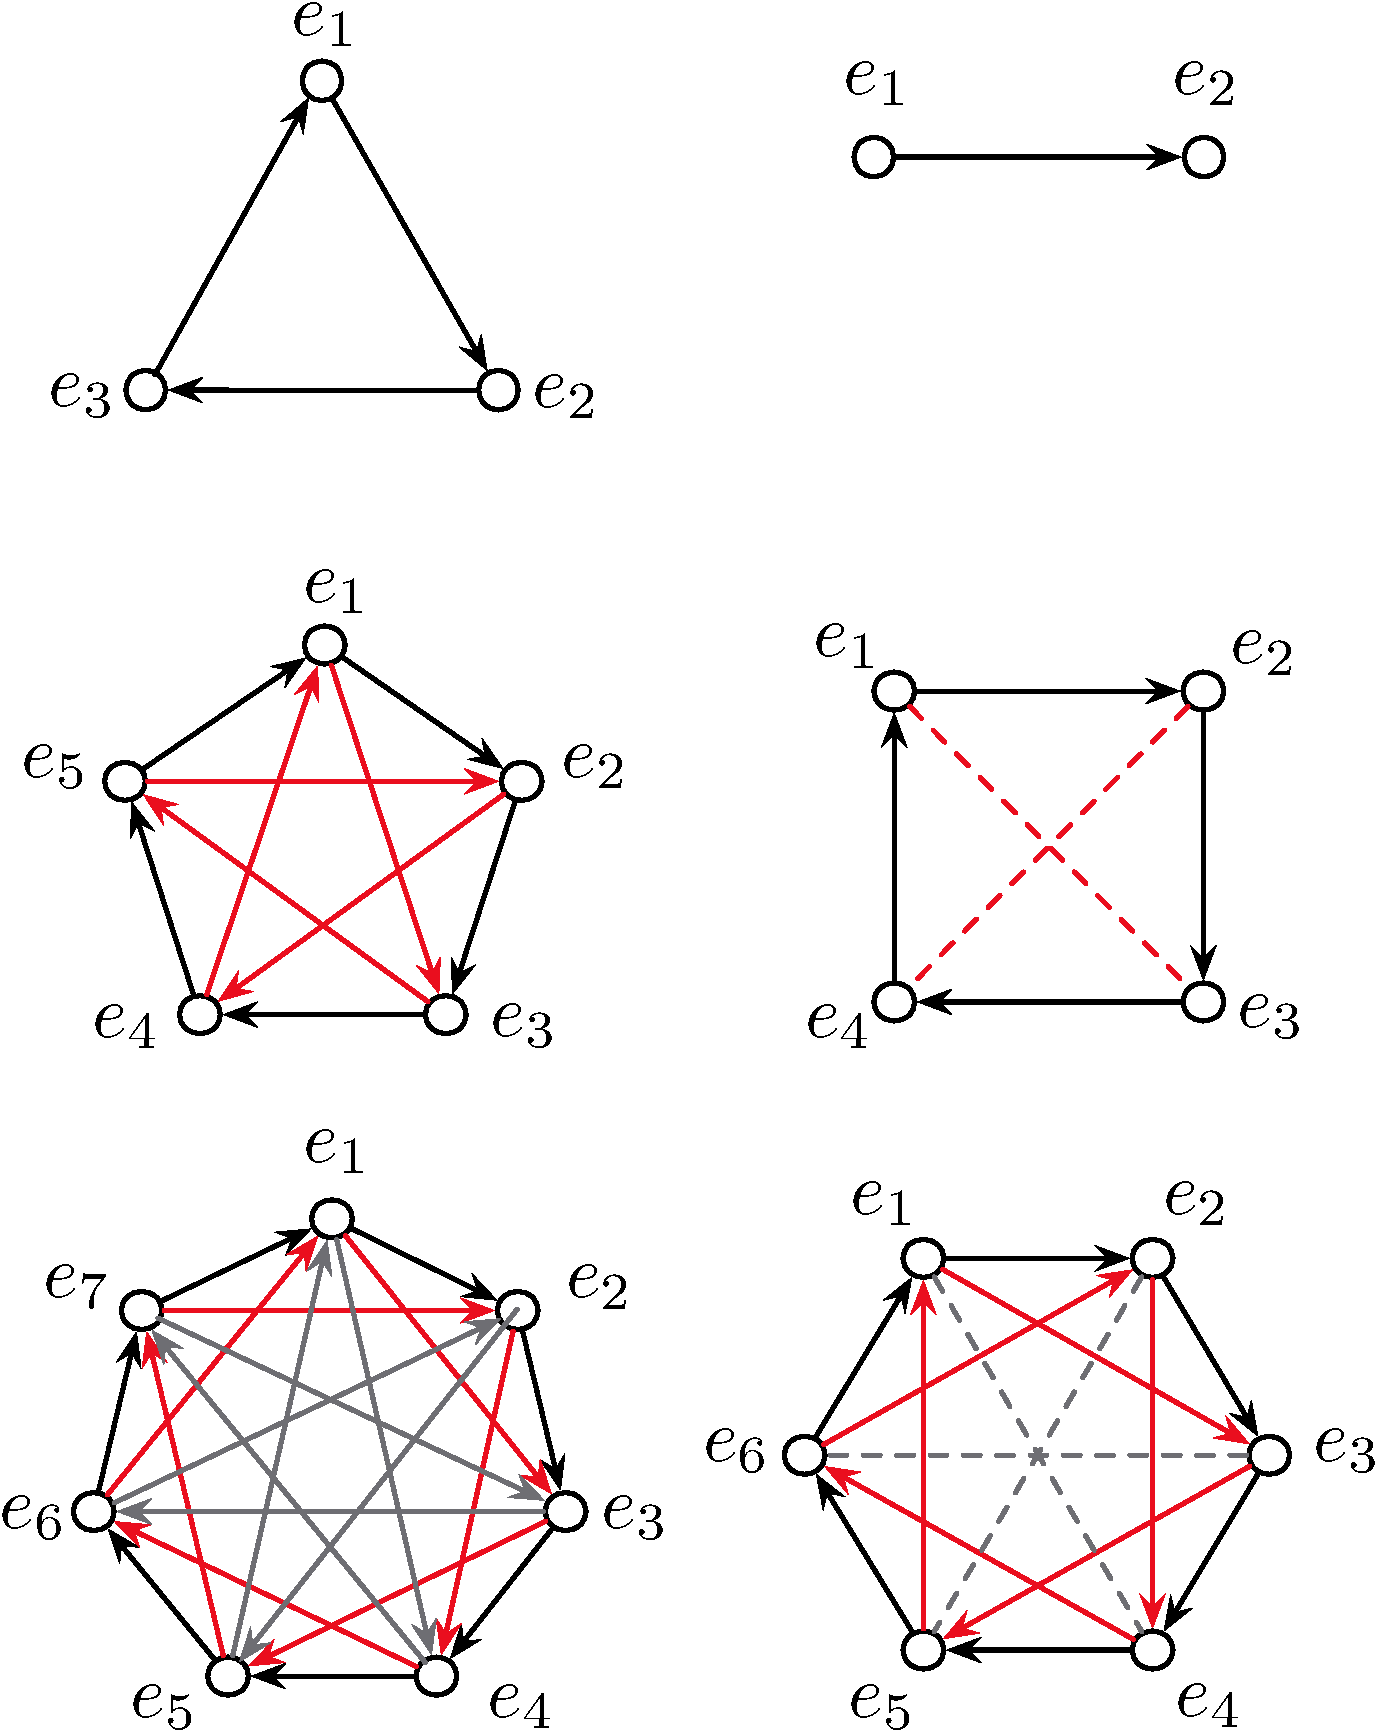
\includegraphics[width=.75\textwidth]{CyclicSymmetricGraphs.pdf}
\caption{A complete graph with $n$ nodes consists of the convex $n$-gon and its inscribed stars. When $n$ is odd, this graph can be turned into a directed graph that is symmetric with respect to cyclic permutations of the basis numbering, but when $n$ is even, the degenerate star, or ``cross" at the center of the graph prevents the construction of a cyclically symmetric directed graph. Because construction of bivector bases is equivalent to construction of complete directed graphs, cyclically symmetric bivector bases can thus only be constructed on odd-dimensional spaces.}
\label{fig:polygonandstars}
\end{center}
\end{figure}



%\begin{theorem}{There are $2^{(n-1)/2)} (\frac{n-1}{2} -1)!  (n-2)!$ distinct cyclic bivector bases that can be constructed on an $n$-dimensional space.}

\begin{theorem}{There are $2^{(n-1)/2} (n-2)!$ distinct cyclic bivector bases that can be constructed on an $n$-dimensional space.} \label{thm:numberofcyclicbivectorbases}

Proof: The polygon and its inscribed stars are together $\frac{n-1}{2}$ loops, which can individually be traversed in any direction, for a total of $2^{(n-1)/2}$ loop sign combinations. 
%There are $(\frac{n-1}{2} -1)!$ cyclic order permutations in which the polygon stars can be traversed. 
Taking the first two points as fixed, there are $(n-2)!$ order-permutations of the other points. (Taking only the first point as fixed would double-count with some of the sign reversals.)% or star-order swaps.)

\end{theorem}

\begin{figure}[tbp]
\begin{center}
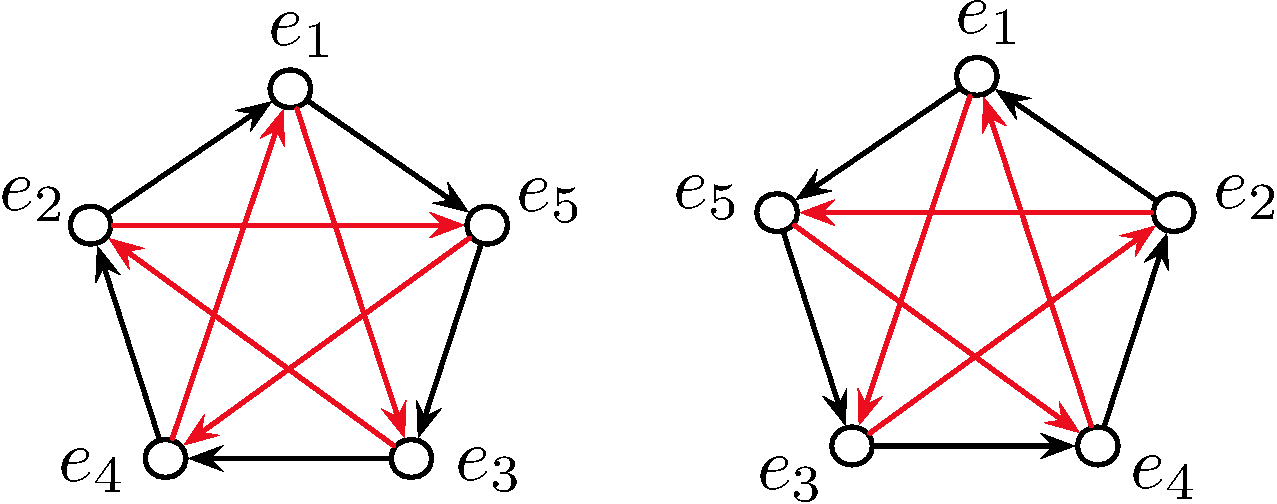
\includegraphics[width=.75\textwidth]{NoNeedToPermute2.pdf}\\
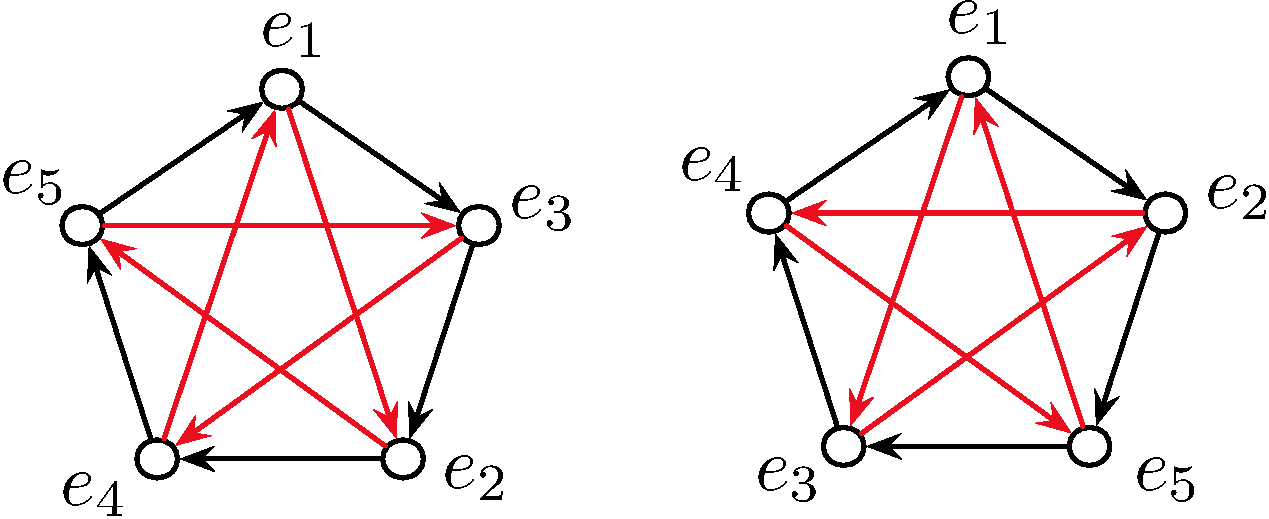
\includegraphics[width=.75\textwidth]{NoNeedToPermute2altalt.pdf}
\caption{%When calculating the number of independent cyclic bivectors we can construct on a space, we can fix one edge of the graph (the selection of $\bv[1]$ and $\bv[2]$ as a reference, and thus and only need to consider permutations of the remaining $n-2$ basis vectors. 
Permutations that change the choice of $\bv[2]$ produce the same directed graph as is produced by some combination of permutations of the $n-2$ other nodes and flipping the signs with which the polygon and stars are traversed. For example, on a five-dimensional space, (top) swapping $\bv[2]$ and $\bv[5]$ while maintaining the directions of both cycles is equivalent to swapping $\bv[3]$ and $\bv[4]$ while flipping the directions of both the pentagon and the pentagram, and (bottom) swapping $\bv[2]$ and $\bv[5]$ and maintaining the directions of both cycles is equivalent to swapping $\bv[3]$, $\bv[4]$, and $\bv[5]$ while flipping the direction of the pentagram.
}
\label{default}
\end{center}
\end{figure}


\section{Cross product}

The standard requirements for a cross product are that it is

Bilinear, orthogonal, and have magnitude equal to the product of the magnitudes when the input vectors are orthogonal, with consequences of anticommutativity and the other identities

In the context of our bivector basis discussion above, we can equivalently describe a cross product as an operation that assigns a basis vector to each basis bivector, $\bp{\bv[i]}{\bv[j]} \rightarrow \bv[k], k\neq i,j$. For geometric consistency under cyclic relabeling of the basis vectors, both the construction of the basis and the assignment must be rotationally symmetric on the graph. All such constructions correspond to assigning a cyclic order to the inscribed stars on the graph and a traversal direction for each, then for each bivector edge in one star, finding $\bv[k]$ by continuing one edge from $\bv[j]$ in the next star.

\subsection{Spaces that could admit a cross product}

\begin{theorem}{Cross products can only be constructed on spaces with ``doubly odd" dimensions.}

Proof: Assigning a rotationally invariant cyclic ordering to a set requires that the set have an odd number of elements, because with an even number of elements it is undefined which of two diametrically opposed points is ``before" the other. The there are $\frac{n-1}{2}$ polygon and stars on an $n$-dimensional space, and therefore they can only be assigned a symmetric cyclic ordering when $\frac{n-1}{2}$  is odd and $n$ is thus ``doubly odd".

\end{theorem}
%On an odd-dimensional space where $\frac{n-1}{2}$ is also odd (which we call ``doubly odd-dimensional"), the polygon and stars in the complete graph can be assigned a rotationally invariant cyclic order (following the same logic as discussed above in the construction of bivectors). If $\frac{n-1}{2}$ is even and not equal to two, then there is no way to assign a rotationally cyclic order to the polygon and stars

%This construction immediately restricts the set of spaces that could have a vector cross product from ``odd-dimensional spaces" to ``odd-dimensional spaces with an even number of inscribed stars" such that the polygon and stars are odd-numbered and can be given a proper cyclic order. (5-D is a special case as it admits a cyclic ordering 1->2 and 2->1, but the next condition prevents the construction of a 5-D cross product.


\subsection{Collisions when attempting to construct a cross product}
There are $ (\frac{n-1}{2} -1)! $ possible polygon-star orderings that we can use to construct the cross product. Together with the direction- and basis-ordering permutations identified in Theorem~\ref{thm:numberofcyclicbivectorbases}, there are $2^{(n-1)/2)} (\frac{n-1}{2} -1)!  (n-2)!$ possible ways in which we could possibly construct a cross product.
Not all of these  direction-star-basis orderings produce valid cross products. Many have ``collisions" in which two bivectors containing a shared basis vector are assigned the same output vector (up to a sign),
%
\begin{equation}
\bp{\bv[i]}{\bv[j]} \rightarrow \bv[k] \qquad \mathrm{and} \qquad \bp{\bv[i]}{\bv[\ell]} \rightarrow \pm\bv[k] 
\end{equation}
%
A ``cross product" incorporating such an assignment would result in a product
%
\begin{equation}
\bv[i] \times (\bv[j]+\bv[\ell]) = 2 \bv[k] \qquad \mathrm{or} \qquad \bv[i] \times (\bv[j]+\bv[\ell]) = 0,
\end{equation}
neither of which is compatible with the condition that the magnitude of the products must be equal to the product of the magnitudes when the inputs are orthogonal, as
\begin{equation} 
1 \cdot \sqrt{2} \neq 2 \qquad \mathrm{and} \qquad 1 \cdot \sqrt{2} \neq 0 .
\end{equation}


Such collisions occur when there exists a single directed star for which traversing a single edge produces the same transformation as is produced by traversing one edge on each of a consecutive pair of directed stars.

The conditions for this lack of overlapping sums are easily checked for the lowest-dimensional doubly-odd-dimensioned spaces:

\paragraph{Three dimensions.} In three dimensions, the polygon-star set is just the polygon and it is its own ``next item" in the polygon-star ordering.. This polygon can be followed in either direction, such that the candidate cross product sequences and their collision tests are
\begin{equation}
\begin{array}{c|c|c}
\text{Polygon-star sequence} & \text{Collision tests} & \text{Validity} \\\hline\hline
\phantom{-}1 & 1+1 = 2 & \text{Pass} \\
2 & 2 + 2 = 4 \equiv 1 &  \text{Pass}
\end{array}
\end{equation}
%
and so three-dimensional spaces admit the construction of two cross products, distinguished by the order in which the basis elements are traversed: $\bv[1]\times\bv[2]=\bv[3]$ and $\bv[1]\times\bv[2]=-\bv[3]$.


\paragraph{Five dimensions.}
In five dimensions, the polygon-star set is the pentagon and the pentagram, and cross product candidates assign to each leg of the pentagon the point reached by following the next leg of the pentagram, and vise versa. This construction means that all cross-product candidates on a five-dimensional space are self-colliding, with pairs of cross products $\bv[i]\times\bv[j1]$ and $\bv[i]\times\bv[j2]$ both mapping to the same $\bv[k]$, as illustrated in Fig.~\ref{fig:5collision} for the positively oriented pentagon cases. The full set of collision tests for the five-dimensional case is
%
\begin{equation}
\begin{array}{c|c|c}
\text{Polygon-star sequence} & \text{Collision tests} & \text{Validity} \\\hline\hline
12 & \begin{bmatrix}1+2= 3 \\ 2+1=3 \end{bmatrix} & \text{Fail} \\
13 & \begin{bmatrix}1+3= 4 \\ 3+1=4 \end{bmatrix} &  \text{Fail} \\
42 & \begin{bmatrix}4+2= 6\equiv{1} \\ 2+4=6\equiv{1} \end{bmatrix} & \text{Fail} \\
43 & \begin{bmatrix}4+3= 7\equiv{2} \\ 3+4=7\equiv{2} \end{bmatrix} &  \text{Fail} \\
\end{array}
\end{equation}

\begin{figure}[htbp]
\begin{center}
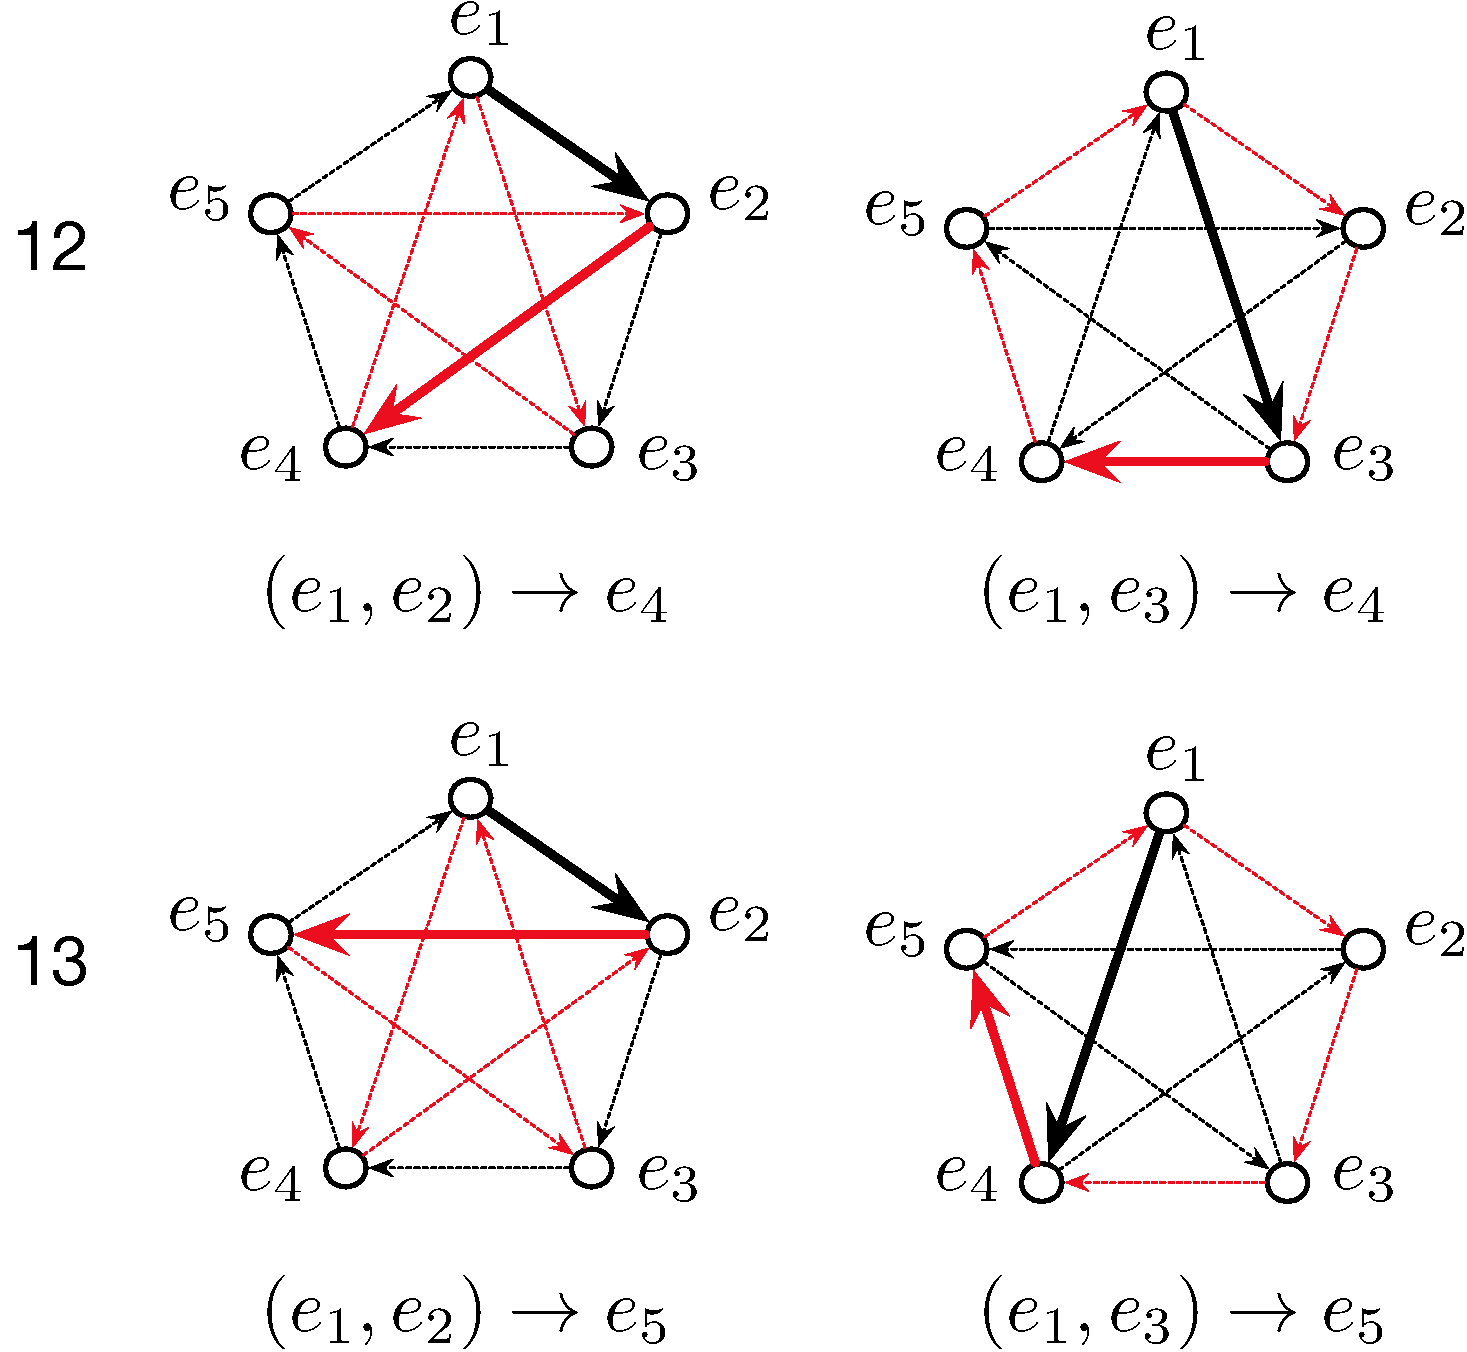
\includegraphics[width=.85\textwidth]{Collisions5D.pdf}
\caption{All cross-product candidates on a five-dimensional space are self-colliding, because they involve moving once along the polygon and once along the pentagram, in the same direction for both pentagon legs and both pentagram legs}
\label{fig:5collision}
\end{center}
\end{figure}



\paragraph{Seven dimensions.} In seven dimensions (the next-smallest doubly-odd space), there are two stars: a ``wide" star in which each edge increases the index count by two or by five (negative two in a seven-element cycle), and a ``narrow" star which increases the index count by three or four. The candidate cross products and their collision tests with the polygon counting forward and a polygon-wide narrow order are
\begin{equation}
\begin{array}{c|c|c}
\text{Polygon-star sequence} & \text{Collision tests} & \text{Validity} \\\hline \hline
1 2 3 & 1+2 = 3 & \text{Fail} \\% \hline 
1 2 4 & \begin{bmatrix} 1+2=3 \\ 2+4=6 \\ 4+1 = 5 \end{bmatrix} &  \text{Pass}\\
1 5 3 & 5+3=8\equiv1 & \text{Fail} \\
1 5 4 & 4+1=5 & \text{Fail} \\
\end{array}
\end{equation}
with only a single candidate producing a valid cross product,
\begin{subequations}
\begin{align}
\bv[i]\times\bv[i+1] = \bv[i+3] \\
\bv[i]\times\bv[i+2] = \bv[i+6] \\
\bv[i]\times\bv[i+4] = \bv[i+6]
\end{align}
\end{subequations}

\begin{figure}[htbp]
\begin{center}
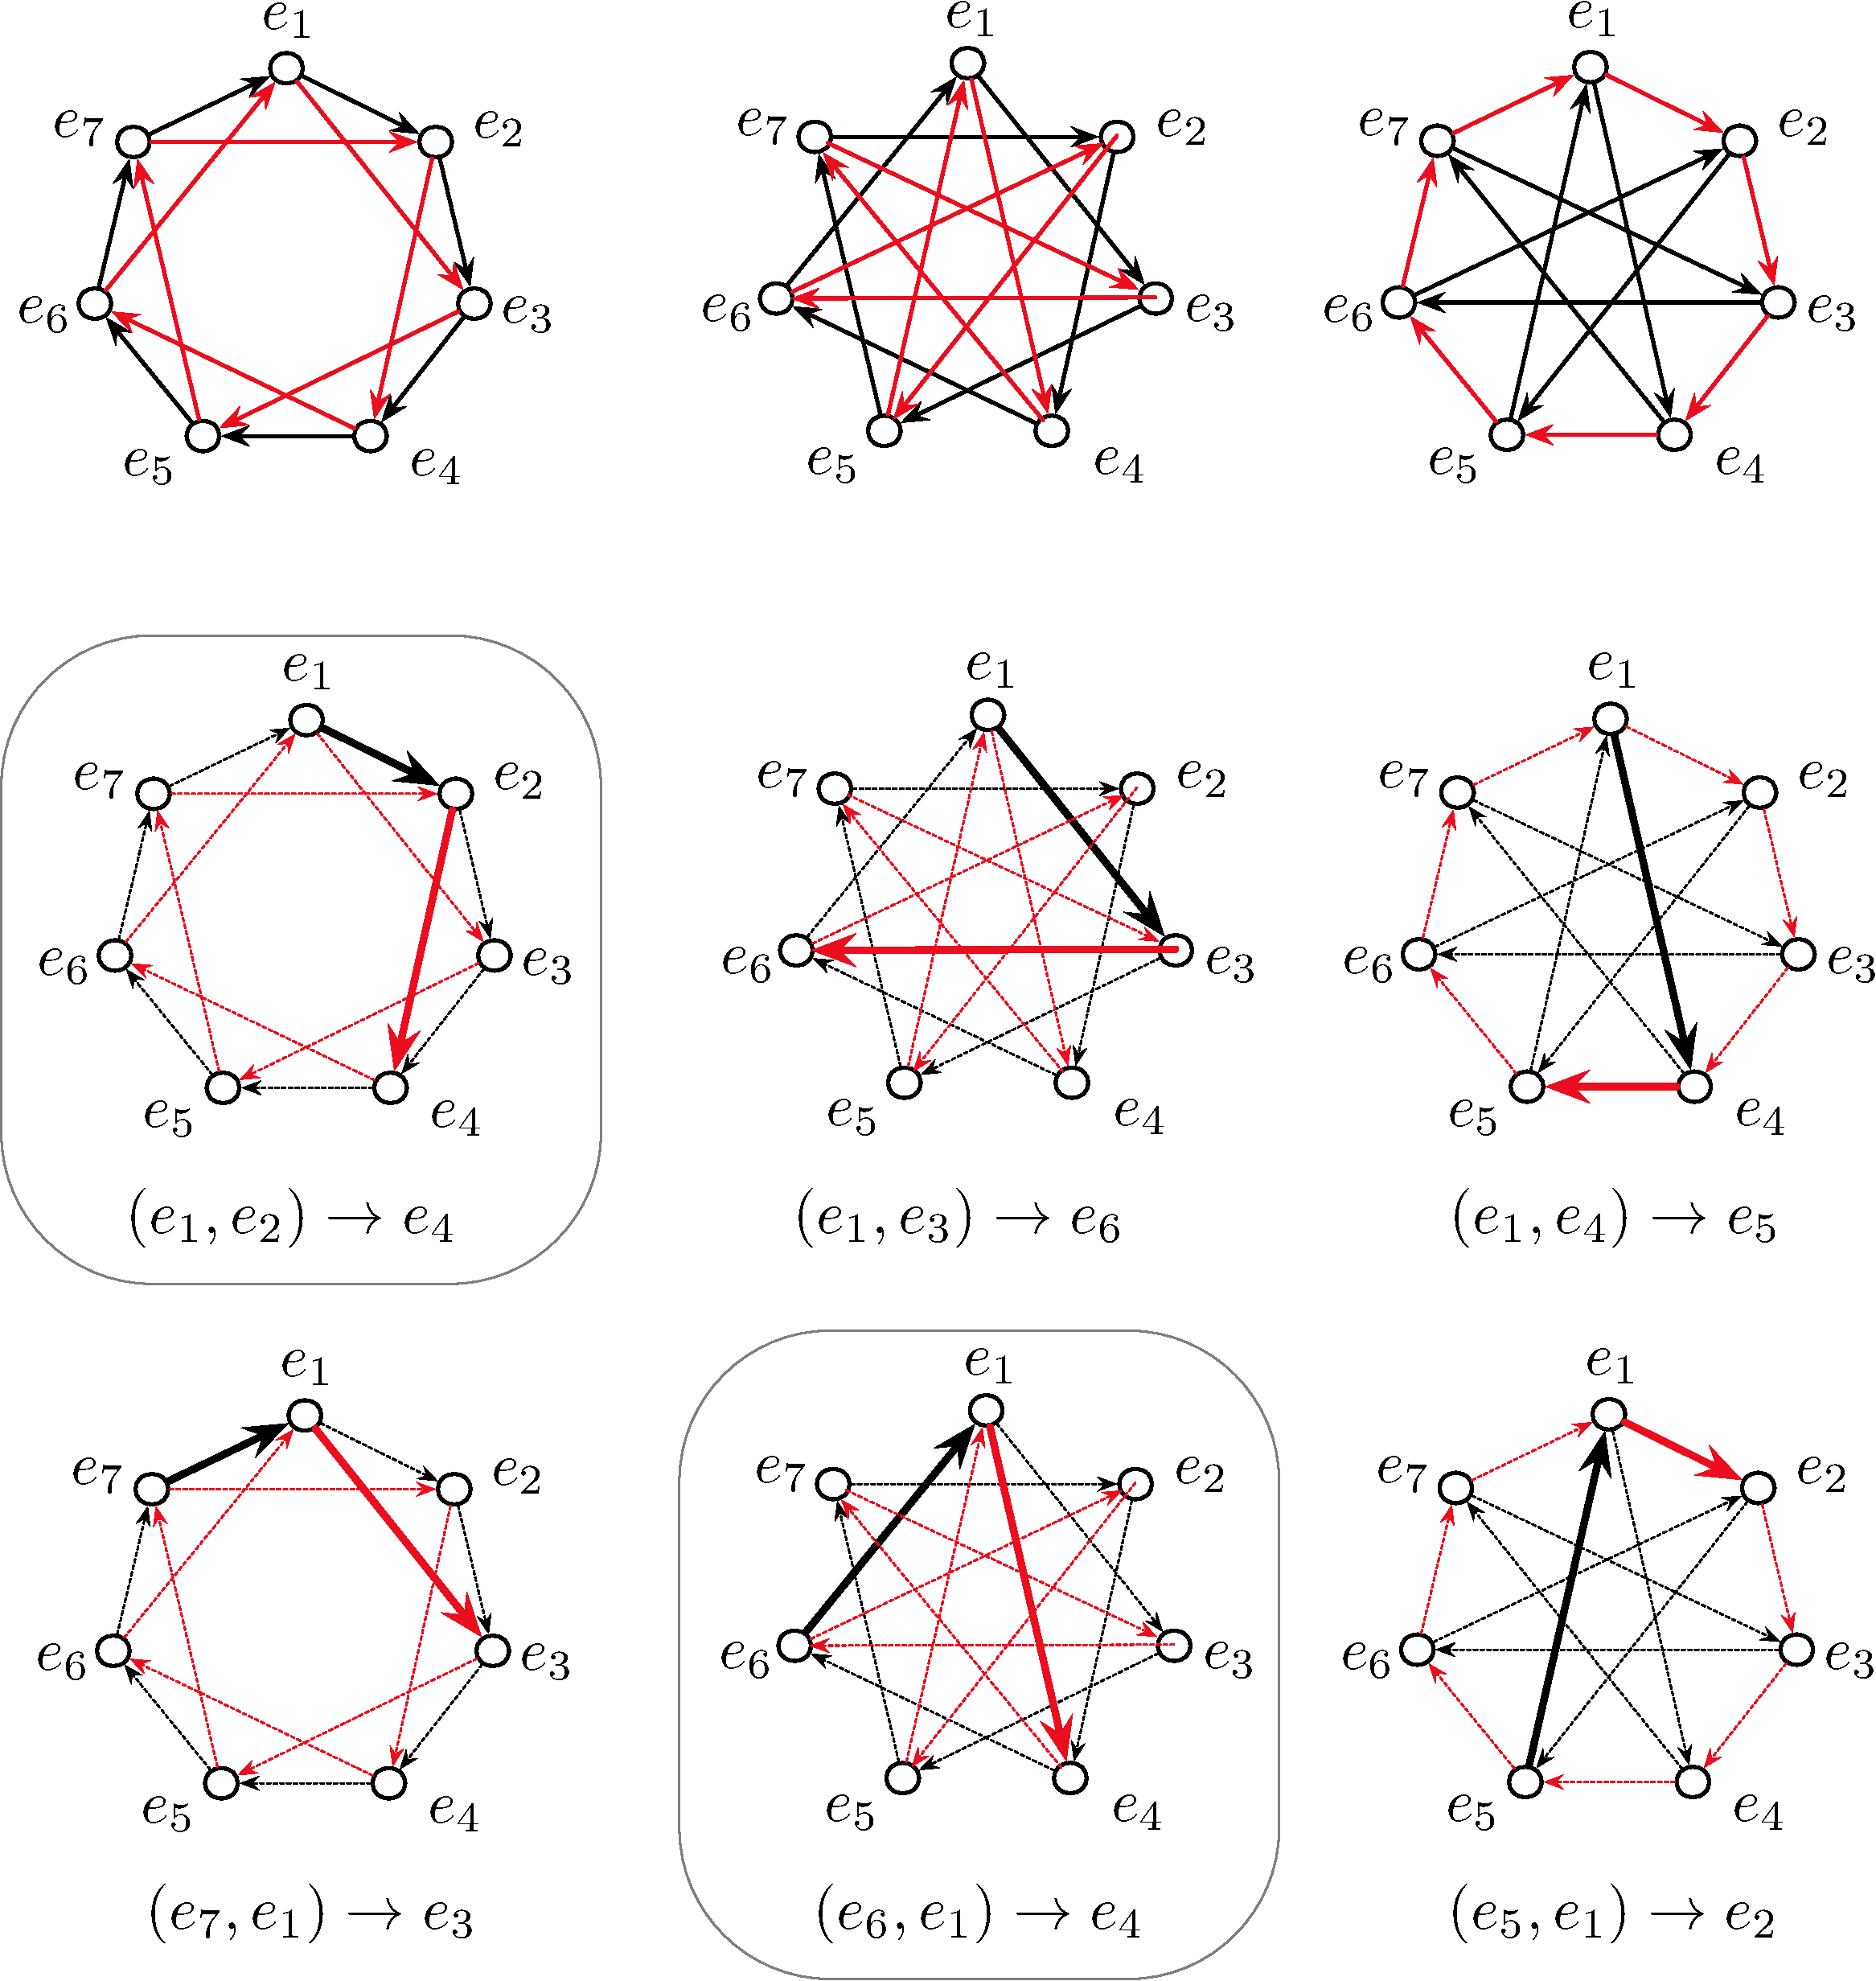
\includegraphics[width=.85\textwidth]{Collisions7D.pdf}
\caption{Some cross-product candidates on a seven-dimensional space are self-colliding, with the cross products whose first and second arguments are $\bv[i]$ both producing the same output basis element. Here, with a polygon-star ordering $123$, both $\bv[1]\times\bv[2]$ and $\bv[6]\times\bv[1]$ map to $\bv[4]$, meaning that this ordering does not define a valid cross product.}
\label{fig:7collision}
\end{center}
\end{figure}

\begin{figure}[htbp]
\begin{center}
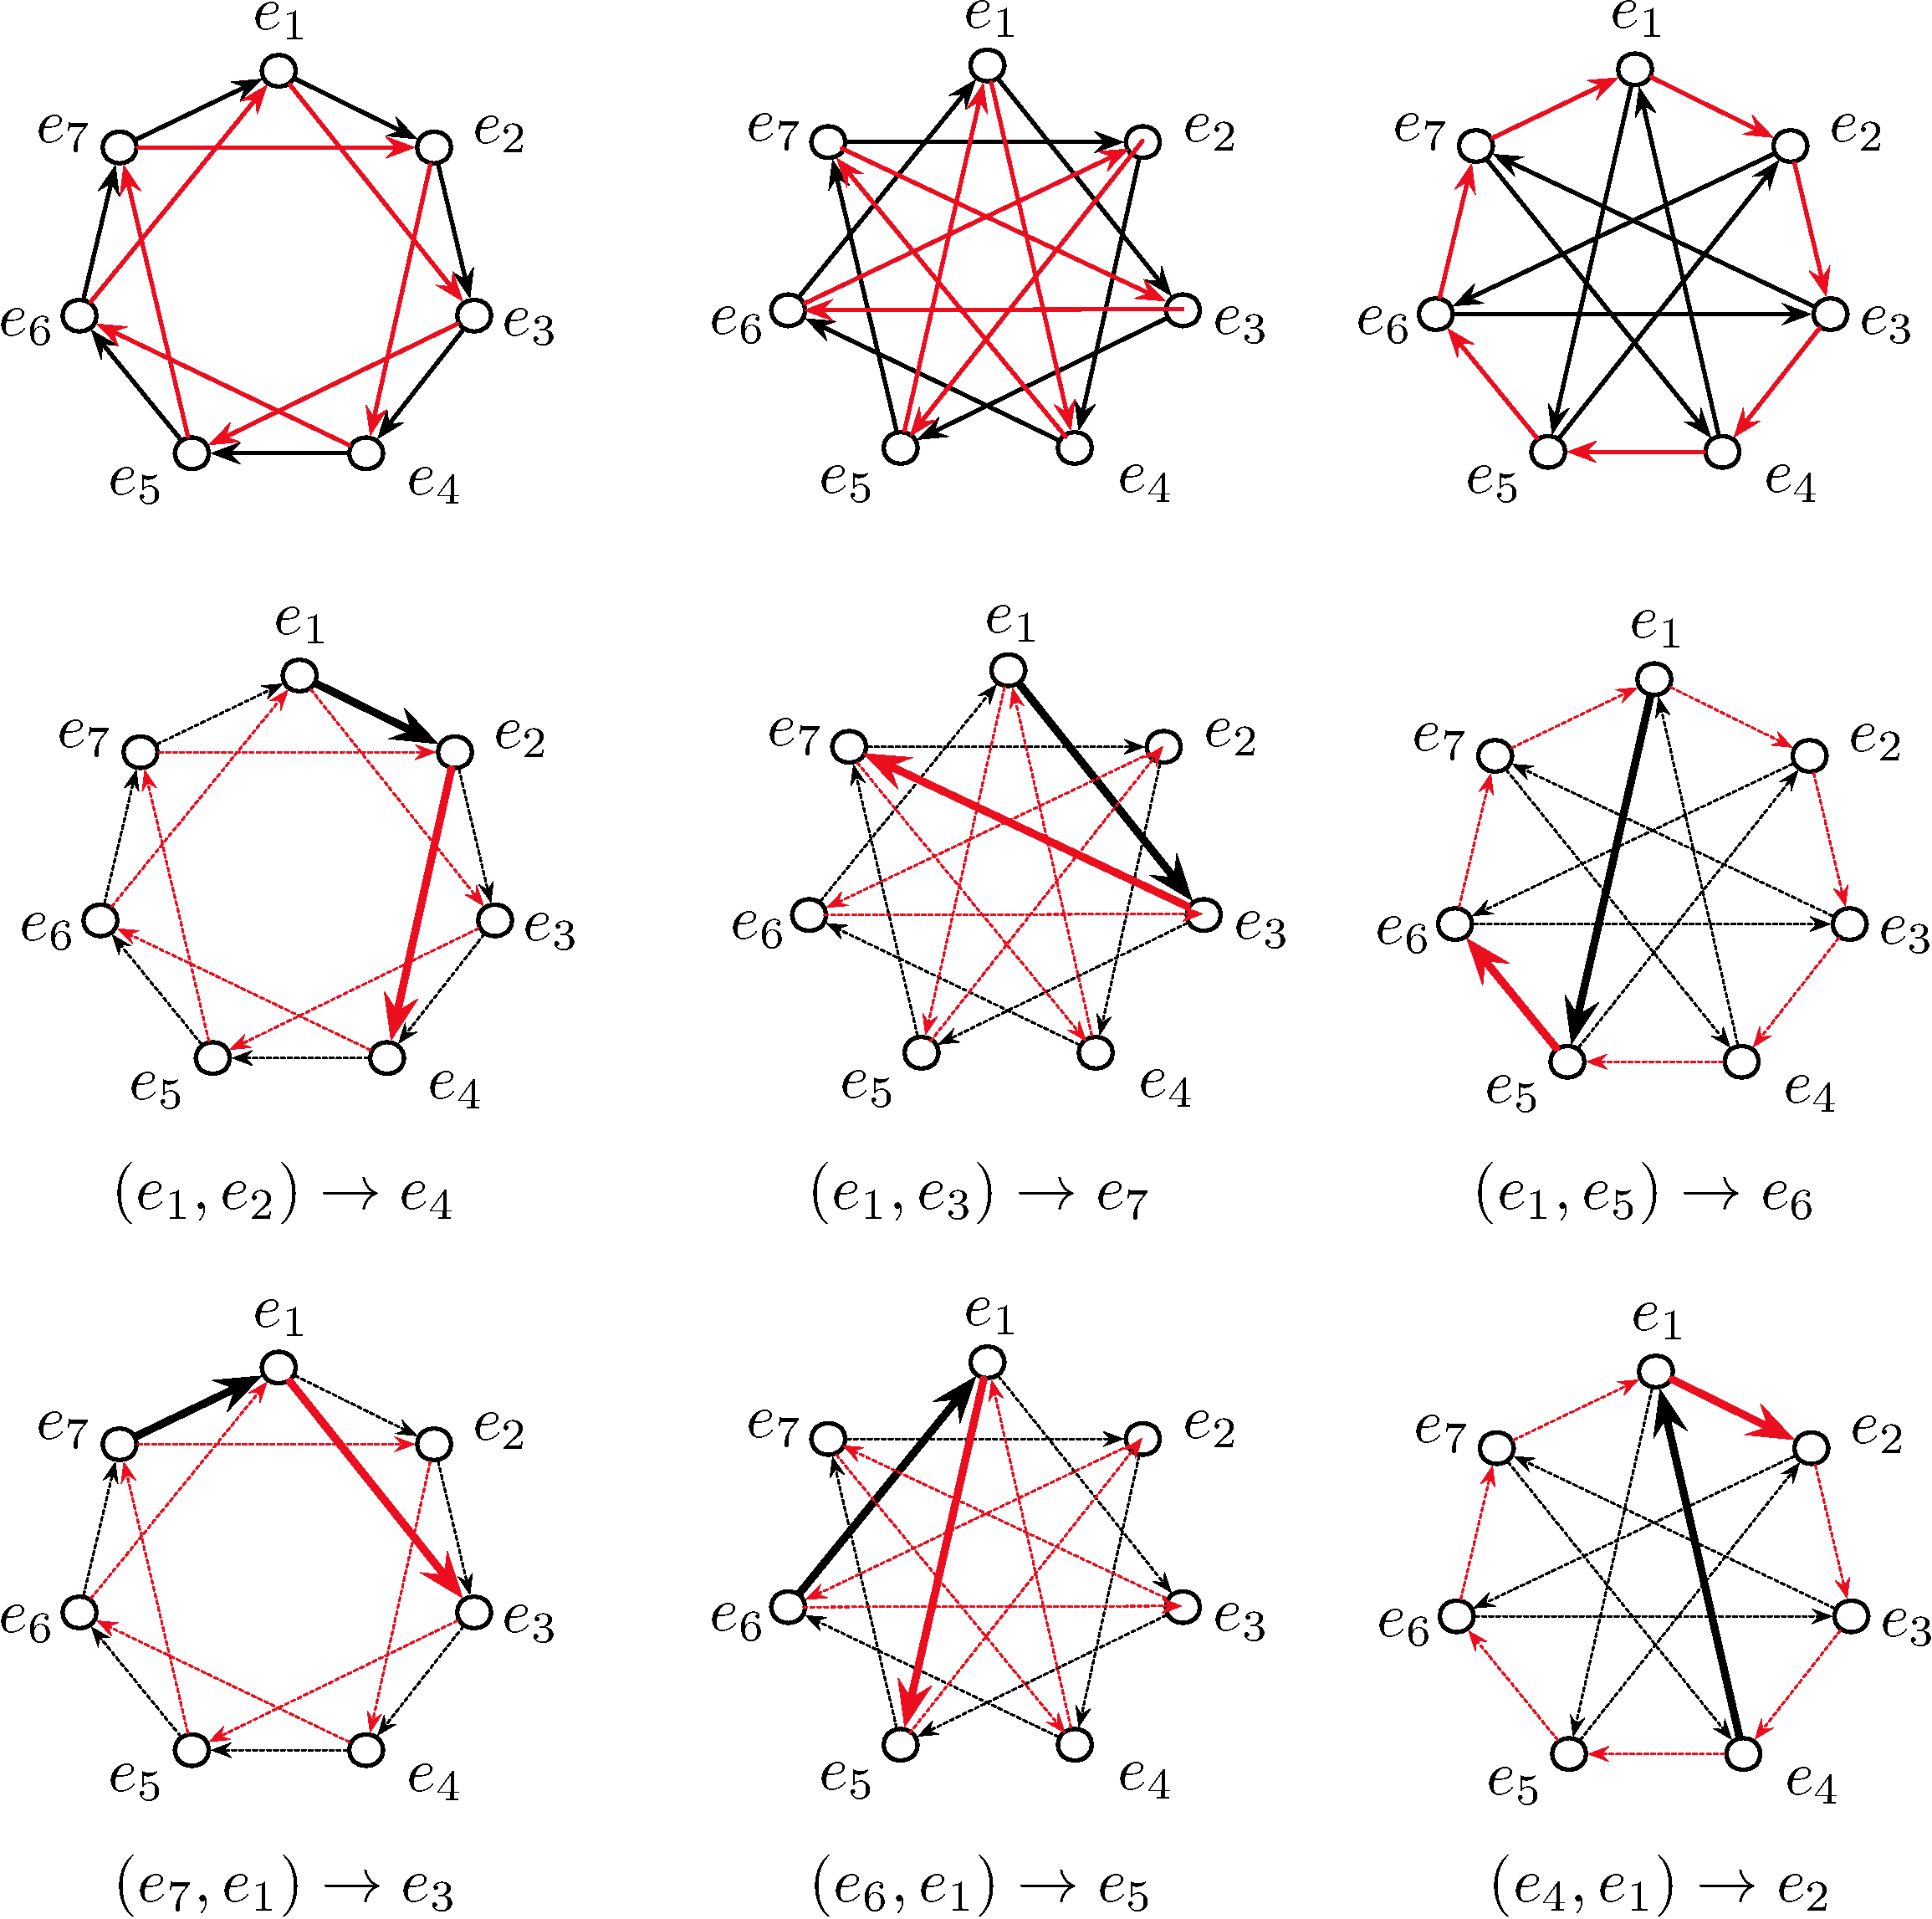
\includegraphics[width=.85\textwidth]{NoCollisions7D.pdf}
\caption{Changing the polygon-star ordering from $123$ to $124$ eliminates the collision, making each cross}
\label{fig:7nocollision}
\end{center}
\end{figure}

Changing the direction of the polygon traversal,
\begin{equation}
\begin{array}{c|c|c}
\text{Polygon-star sequence} & \text{Collision tests} & \text{Validity} \\\hline \hline
6 2 3 & 1+2 = 6+3=9\equiv2 & \text{Fail} \\% \hline 
6 2 4 & 2+4=6 & \text{Fail}\\
6 5 3 &  \begin{bmatrix} 6+5=11\equiv4 \\ 5+3=8\equiv1 \\ 3+9=9\equiv2 \end{bmatrix} &  \text{Pass} \\
6 5 4 &6+5=11\equiv4 & \text{Fail} \\
\end{array}
\end{equation}
 again leaves only a single candidate that produces a valid cross product,
 \begin{subequations}
\begin{align}
\bv[i]\times\bv[i+6] = \bv[i+4] \\
\bv[i]\times\bv[i+5] = \bv[i+1] \\
\bv[i]\times\bv[i+3] = \bv[i+2],
\end{align}
\end{subequations}
 which is the sign reversal of all traversals in the original passing candidate.

Changing the order of the polygon-star sequences as
\begin{equation}
\begin{array}{c|c|c}
\text{Polygon-star sequence} & \text{Collision tests} & \text{Validity} \\\hline \hline
1 3 2& 1+2 = 3 & \text{Fail} \\% \hline 
1 4 2 & \begin{bmatrix} 1+2=3 \\ 2+4=6 \\ 4+1 = 5 \end{bmatrix} &  \text{Pass}\\
1 3 5  & 5+3=8\equiv1 & \text{Fail} \\
1 4 5 & 4+1=5 & \text{Fail} \\
\end{array}
\end{equation}
and
\begin{equation}
\begin{array}{c|c|c}
\text{Polygon-star sequence} & \text{Collision tests} & \text{Validity} \\\hline \hline
6 3 2 & 1+2 = 6+3=9\equiv2 & \text{Fail} \\% \hline 
6 4 2 & 2+4=6 & \text{Fail}\\
6 3 5 &  \begin{bmatrix} 6+5=11\equiv4 \\ 5+3=8\equiv1 \\ 3+9=9\equiv2 \end{bmatrix} &  \text{Pass} \\
6 4 5 &6+5=11\equiv4 & \text{Fail} \\
\end{array}
\end{equation}
 again produces a single valid cross product for each polygon traversal direction,
  \begin{subequations}
\begin{align}
\bv[i]\times\bv[i+1] = \bv[i+3] \\
\bv[i]\times\bv[i+4] = \bv[i+6] \\
\bv[i]\times\bv[i+2] = \bv[i+5],
\end{align}
\end{subequations}
and
\begin{subequations}
\begin{align}
\bv[i]\times\bv[i+6] = \bv[i+4] \\
\bv[i]\times\bv[i+3] = \bv[i+1] \\
\bv[i]\times\bv[i+5] = \bv[i+2],
\end{align}
\end{subequations}
 with the interesting feature that changing the order of the polygon-star sequence, while producing distinct cross products, does not change the set of star directions needed to produce a valid cross product -- all the valid cases are either re-orderings of $124$ or $635\equiv-(124)$.

Taking these validity tests together, we see that the $2^{(7-1)/2)} = 2^(3)$  direction-permutations for bivector pairings on seven-dimensional space are reduced to just $2$ sets of signs that correspond to valid cross products (which is consistent with the two signs we found for the cross product in three dimensions), and that the $(\frac{7-1}{2} -1)! = 2$ permutations of the polygon-star order produce distinct valid cross products. Combining this with the $(7-2)! = 120 $ edge-fixed permutations of the basis ordering, we can conclude that there are
\begin{equation}
2 \cdot 2 \cdot 120 = 480
\end{equation}
valid cross products amongst the 
\begin{equation}
8 \cdot 2 \cdot 120 = 1920
\end{equation}
distinct bivector pairings in seven-dimensional space, which is consistent with previous results in the literature.

\subsection{Higher-dimensional spaces}

Beyond confirming the previous results that geometrically consistent cross products can be defined in seven dimensions, we can extend our reasoning above to also rule out the possibility of such a cross product existing in dimensions greater than seven.

Based on the  analysis, we can restrict our attention to direction-order sequences starting with 1 and with stars ordered by their increasing increment when followed in the same direction as the polygon. The general form of such sequences is
%
\begin{equation}
1\hspace{1em}\frac{2}{n-2} \hspace{1em} \frac{3}{n-3}\hspace{1em} \cdots \hspace{1em} \frac{(n-1)/2 -1}{(n-1)/2 +2} \hspace{1em} \frac{(n-1)/2}{(n-1)/2 +1}
\end{equation}
with either the positive (top) or negative (bottom) parity element selected from each pair.


Three conditions on these sequences together ensure that there are no paths through the sequence that produce valid cross products: 
\begin{enumerate}
\item Paths through this sequence that produce valid cross products must alternate parity, because equences that contain consecutive elements with the same parity fail the validity test, because one of those numbers will sum with $1$ to produce the other.
\item Paths through this sequence that produce valid cross products cannot start with $n-2$, because with alternating parity, the next element is $3$, and  $(n-2)+3 \equiv 1$, making these sequences invalid.
\item Paths through this sequence that produce valid cross products cannot start with $2$, because with alternating parity, the last two elements are 
$(n-1)/2 -1$ and $(n-1)/2 +1$ or $(n-1)/2 +2 $ and $(n-1)/2$, both of which are separated by $2$, again making the sequences invalid, and leaving no remaining candidates.
\end{enumerate}
Seven-dimensional spaces escape this fate because $2$ fills the dual role of starting the sequence and acting as the $(n-1)/2 -1$ element in the final pair, such that $2$ is not available to add to $(n-1)/2 -1$ to produce $(n-1)/2 + 1$.

\end{document}


\item Paths through this sequence that produce valid cross products must start with $2$, because alternating sequences starting with $n-2$ have $3$ as the second value, and $(n-2)+3 \equiv 1$, making these sequences fundamentally invalid.
\item For a ``doubly odd" n, alternating sequences starting at 2 end with a ``downstroke",
\begin{equation}
1\hspace{1em} 2\hspace{1em} \ldots \hspace{1em} ((n-1)/2 -1) \hspace{1em} ((n-1)/2 + 1)
\end{equation}
such that these sequences are also fundamentally invalid, and thus that there are no valid cross product sequences for any space with dimension greater than 7.
\end{enumerate}
\end{document}




Any valid path through this sequence must start with 2, because alternating sequences starting with (n-2) have 3 as the second value, and $(n-2)+3 \equiv 1$ making these sequences fundamentally invalid.

For a ``doubly odd" n, alternating sequences starting at 2 end with a ``downstroke",

1, 2, … ((n-1)/2 -1) ((n-1)/2 + 1)

such that these sequences are also fundamentally invalid, and thus that there are no valid cross product sequences for any space with dimension greater than 7.

Seven escapes this fate because ((7-1)/2 -1) = 2, suc

\end{document}

%2^{(n-1)/2)} (\frac{n-1}{2} -1)!
 %and is its own ``next item" in the polygon-star ordering. This means that the 

%, with increment 1 or -1 depending on sign. There are no sums of two increments, so 3 dimensions on an ordered basis admits the construction of two cross products distinguished by the order in which the basis elements are traversed: e1xe2=e3 and e1xe3=e2


\begin{theorem}{

\end{theorem}


These conditions mean that the only direction-and-star orderings that produce valid cross products are those for which the sums of increments of the polygon and stars (the amount by which stepping along one edge increases the index number) do not have any shared positively-oriented sums, and the sum of any two increments is not equal to any single increment.


% such that a cross product starting at a given node has the same value as a different cross product ending at 

%stepping along a polygon or star and then along next polygon or star produces the same nodal increment as does stepping along a single

%polygon or star for which traversing a single edge increments the node index by the same  as is produced by traversing the edges of a pair of stars

%Such collisions occur under two conditions:
%
%1. There are two pairs of directed polygons/stars for which starting at a node and traversing each star by one edge results in the same transformation
%2. There exists a single star for which traversing a single edge produces the same transformation as is produced by traversing the edges of a pair of stars


The conditions for this lack of overlapping sums are easily checked over candidate values:

In 3 dimensions, there is just the polygon, with increment 1 or -1 depending on sign. There are no sums of two increments, so 3 dimensions on an ordered basis admits the construction of two cross products distinguished by the order in which the basis elements are traversed: e1xe2=e3 and e1xe3=e2

In 5 dimensions, candidate cross products correspond to defining the polygon-edge cross products by following the next edge on the star and vise versa. Polygon-star and star-polygon traversals on this graph are always equivalent to each other, so there are no collision free cross-product candidates in 5 dimensions.

Numerically, the signed options for the polygon and the star give this system increment numbers of (1 or 5, 2 or 3), with increment sequences and their sums

1 2 | 1+2 = 3 | 2+1 =3
1 3 | etc
5 3
5 

(Note that in this space, 1-2 and 2-1 are distinct positively-oriented sequences, so we sum both of them.) The sums are equal to each other, disqualifying any of these candidates for the cross product.

In 7 dimensions, the candidates under a polygon-wide-narrow ordering are (1 or 6, 2 or 5, 3 or 4) and for the polygon-narrow-wide ordering are (1 or 6, 3 or 4, 2 or 5). Their test conditions are

Polygonal, wide, narrow
1 2 3  -> 1+2 = 3 Fail
1 2 4 -> 1+2 =3, 2+4= 6, 4+1= 5 Pass
1 5 3 -> 3+5 = 8 \equiv 1 Fail
1 5 4 -> 4+1 = 5 Fail

6 2 3 -> 3+6 = 9 \equiv 2 Fail
6 2 4 -> 2+4 = 6 Fail
6 5 3 -> 6+5 = 11 \equiv 4, 5+3 = 8 \equiv 1, 
6 5 4 -> 6+5 = 11 \equiv 4 Fail

Polygon, narrow, wide
1 3 2
1 4 2 Pass
1 3 5
1 4 5

6 3 2
6 4 2
6 3 5 Pass
6 4 5

Note that the pass-fail criteria are invariant with respect to the cyclic ordering of the polygons, so we don’t actually need to take the order of the pairings into account in our test (though the cyclic ordering is a necessary precondition for a valid cross product, and the different cyclic orderings result in distinct cross products).

The 6-starting valid sequences are reflections of the 1-starting valid sequences, so, while these are again distinct sequences, we don’t need to consider them explicitly when looking for valid cross product sequences.

Also note that the pass cases are those for which the 1-starting (positively oriented) sequences have elements taken from the Fibonacci-minus-1 sequence.

—
Higher dimensional spaces

Based on the above analysis, we can restrict our attention to direction-order sequences starting with 1 and with stars ordered by their increasing increment when followed in the same direction as the polygon. The general form of such sequences is

1 2 (n-2) 3 (n-3) … … ((n-1)/2 -1) ((n-1)/2 +2) (n-1)/2 ((n-1)/2 +1)

with either the positive or negative parity element selected from each pair.

Valid paths through this sequence must alternate parity: Sequences that have consecutive numbers in it with the same parity fail, because one of those numbers will sum with 1 to produce the other. 

Any valid path through this sequence must start with 2, because alternating sequences starting with (n-2) have 3 as the second value, and $(n-2)+3 \equiv 1$ making these sequences fundamentally invalid.

For a ``doubly odd" n, alternating sequences starting at 2 end with a ``downstroke",

1, 2, … ((n-1)/2 -1) ((n-1)/2 + 1)

such that these sequences are also fundamentally invalid, and thus that there are no valid cross product sequences for any space with dimension greater than 7.

Seven escapes this fate because ((7-1)/2 -1) = 2, such that 2 is not available to add to ((n-1)/2 -1) to produce ((n-1)/2 + 1).

\end{document}